%!TEX root = main_ISMB.tex
\section{Supplementary data}
\subsection{Benchmark \ourprog vs \RNAinverse}
Using the same dataset of $50$ structures, we generated $100$ samples
per structure with \RNAinverse. They yield for most parameters
a high entropy.
Table.~\ref{tab:nb_rnainv} contains the number of sample with a given \GCContent generated by \RNAinverse. The vast majority resides around $50\%-70\%$, showing one of its major deficiencies. 
 For all structures that have been solved 
by the three methods, only \RNAinverse, only \texttt{Incarnation} and
\texttt{Incarnation} followed by \RNAinverse, 
we present for every different concentration of \GCContent
the average sample entropy. and the average base pairs entropy in Figure.~\ref{fig:rnainverse}.

\begin{table}[h!]
	\begin{center}
		\begin{tabular}{|c|ccccc|}
		\hline
		Target \GCContent & 10 & 30 & 50 & 70 & 90\\ \hline
   $\#$\RNAinverse samples& 11 & 437 & 3362 & 1155 & 35\\ \hline
		\end{tabular}
	\end{center}
  \caption{Overall \GCContent distribution for sequences designed using \RNAinverse.}
	\label{tab:nb_rnainv}
\end{table}


\begin{figure}[ht!]
	\centering
	%\hspace{-5em}
	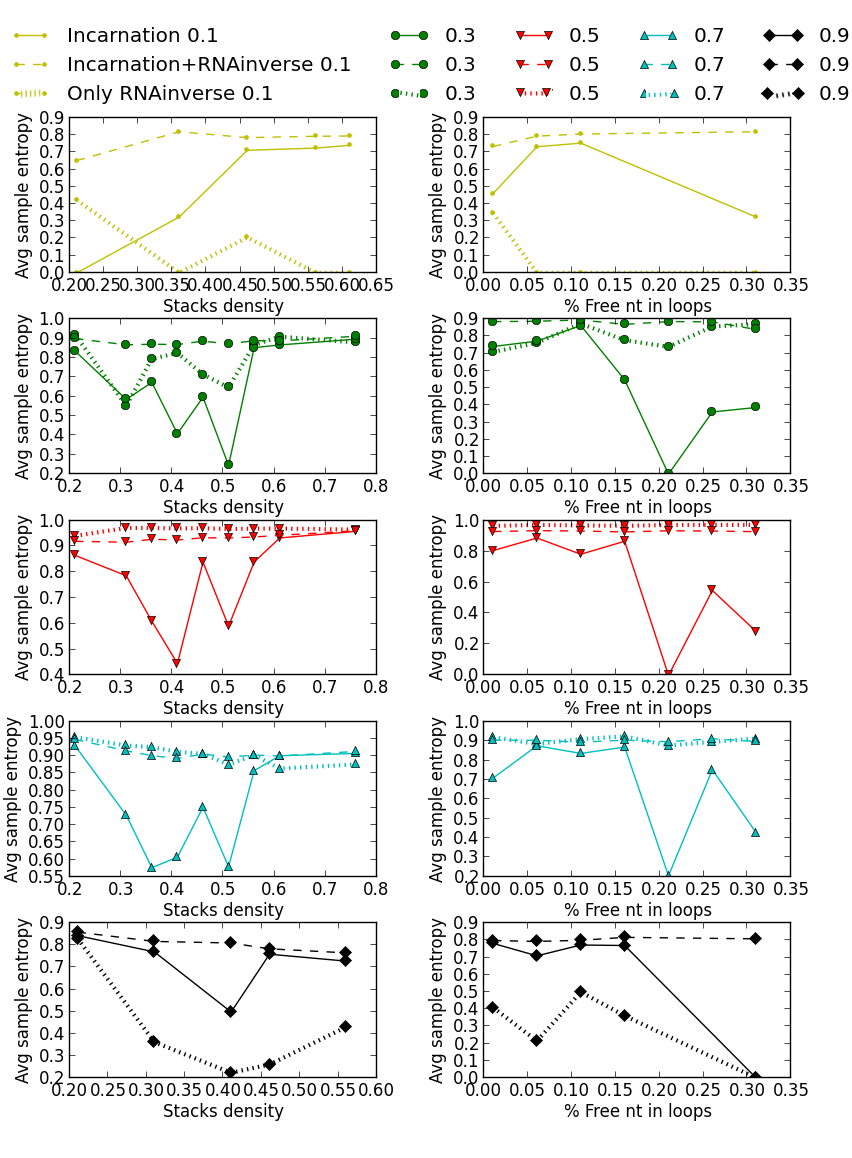
\includegraphics[scale=0.4]{Figures/RNAinverse_data_100.png}
	\caption{Entropy and \GCContent  for structures solved by
	the 3 methods.}
	\label{fig:rnainverse}
\end{figure}
{\em Récupérer Base-pair entropy}


%The same analysis but only for structures solved by \texttt{Incarnation}
%and \texttt{Incarnation} followed by \RNAinverse, is presented in 
%Fig.~\ref{fig:inc_rnainv}
%
%\begin{figure}
%	\centering
%	\includegraphics{}
%	\caption{Entropy and \texttt{C+G} content for structures solved by
%	the \texttt{Incarnation} and \texttt{Incarnation}$+$\RNAinverse.}
%	\label{fig:inc_rnainv}
%\end{figure}
\subsection{Impact of local search on the \GCContent of \ourprog output}

These data demonstrate that the local search heuristic used to design nucleotides in loop regions has a very limited impact on the \GCContent. For each class of \GCContent, we show in Table~\ref{table:impact_on_gc}, the observed \GCContent of the sequence sampled by \ourprog, and then we report the observed \GCContent after the \RNAinverse step (as defined in Section \ref{subsec:glocal_method}). Our results show that the \GCContent is relatively well conserved. 

\begin{table}[h!]
\begin{center}
\begin{tabular}{|c|c|c|}
\hline
target \GCContent & \ourprog & \ourprog + \RNAinverse \\
\hline
10\% & 0.15 & 0.21\\
30\% & 0.30 & 0.33\\
50\% & 0.48 & 0.49\\
70\% & 0.71 & 0.69\\
90\% & 0.83 & 0.78\\
\hline
\end{tabular}
\end{center}
\caption{Observed \GCContent of solutions returned by \ourprog (2nd column) and after the application of the local search heuristic (3rd column).}
\label{table:impact_on_gc}
\end{table}
